\documentclass[10pt,twocolumn,letterpaper]{article}

\usepackage{amsmath,amssymb,amsthm}
\usepackage{booktabs}
\usepackage{graphicx}
\usepackage{hyperref}
\usepackage{microtype}
\usepackage{tikz}
\usetikzlibrary{arrows.meta,positioning,shapes.geometric}
\usepackage[margin=0.72in]{geometry}

\newtheorem{proposition}{Proposition}

\title{\textbf{VascuMamba-Spot: Continuous-Time Autonomic-Gated Neuro-Vascular and Kinematic State-Space Modeling for Untrimmed Micro-Expression Spotting and Recognition}}

\author{VascuMamba-Spot Authors}
\date{}

\begin{document}
\maketitle

\begin{abstract}
Automated spotting and recognition of facial micro-expressions (MEs) in continuous, untrimmed video remains severely limited by false alarms from non-emotional facial kinematics (spontaneous eyeblinks, swallowing, and rigid head jitter) and the quadratic $O(T^2)$ memory bottleneck of Video Transformers on high-frame-rate streams. We introduce \textbf{VascuMamba-Spot}, a linear-complexity $O(T)$ Bidirectional Selective State-Space architecture grounded in a dual-pathway neuro-vascular hypothesis: while non-emotional eyeblinks produce surface motion without autonomic arousal, genuine suppressed emotions co-activate facial muscle strain and sympathetic cutaneous blood-volume pulse modulation. VascuMamba-Spot extracts physically normalized 12-ROI Cauchy optical strain tensors alongside 7-ROI motion-debiased remote photoplethysmography (rPPG) features, using an autonomic arousal gate $g_t^{\mathrm{aut}}$ to multiplicatively modulate continuous physical-time state discretization $(\Delta_t^{\mathrm{phys}}, B_t^{\mathrm{kin}})$. We further introduce self-supervised neuro-vascular pretraining across unlabeled long videos and privileged BIOPAC-to-rPPG gate distillation on CAS(ME)$^3$, requiring zero wearable sensors at inference. Formal stability bounds, color-space-aware RGB/monochrome pipelines, and standardized Leave-One-Subject-Out (LOSO) benchmarks are established across RGB and monochrome datasets.
\end{abstract}

\section{Introduction}
Facial micro-expressions (MEs) are brief ($40\text{--}500\text{ ms}$), involuntary, low-intensity facial muscle contractions occurring when an individual consciously or unconsciously suppresses genuine affect~\cite{yan2014casme2,davison2018samm}. Accurate automated spotting and recognition hold significant value in affective computing, clinical psychiatry, and human-computer interaction.

However, transitioning from pre-segmented clip recognition~\cite{liong2019ststnet,gan2019offapexnet} to continuous, untrimmed video spotting~\cite{qu2017casme2sq,li2022casme3} exposes two fundamental ceilings:
\begin{enumerate}
  \item \textbf{Kinematic False Alarms:} Purely visual detectors treat MEs strictly as surface pixel motion, causing high false-positive rates on non-emotional facial kinematics (spontaneous eyeblinks, speech micro-movements, and rigid head pose jitter).
  \item \textbf{Quadratic Sequence Bottleneck:} Video Vision Transformers incur $O(T^2)$ self-attention memory overhead on long $200\text{ fps}$ sequences while risking high-variance overfitting on small ME datasets.
\end{enumerate}

\textbf{Core Hypothesis.} Genuine emotional suppression co-activates extrapyramidal facial motor pathways (CN~VII) and Autonomic Nervous System (ANS) sympathetic modulation reflected in peri-suppression cardiac pulse-wave amplitude and inter-beat dynamics. Non-emotional eyeblinks induce surface strain without autonomic arousal. \textbf{VascuMamba-Spot} couples both signals inside a continuous-time Bidirectional Selective State-Space Model (Mamba)~\cite{gu2023mamba} where autonomic arousal multiplicatively gates kinematic state transitions in $O(T)$ time (Fig.~\ref{fig:teaser}).

\begin{figure}[t]
\centering
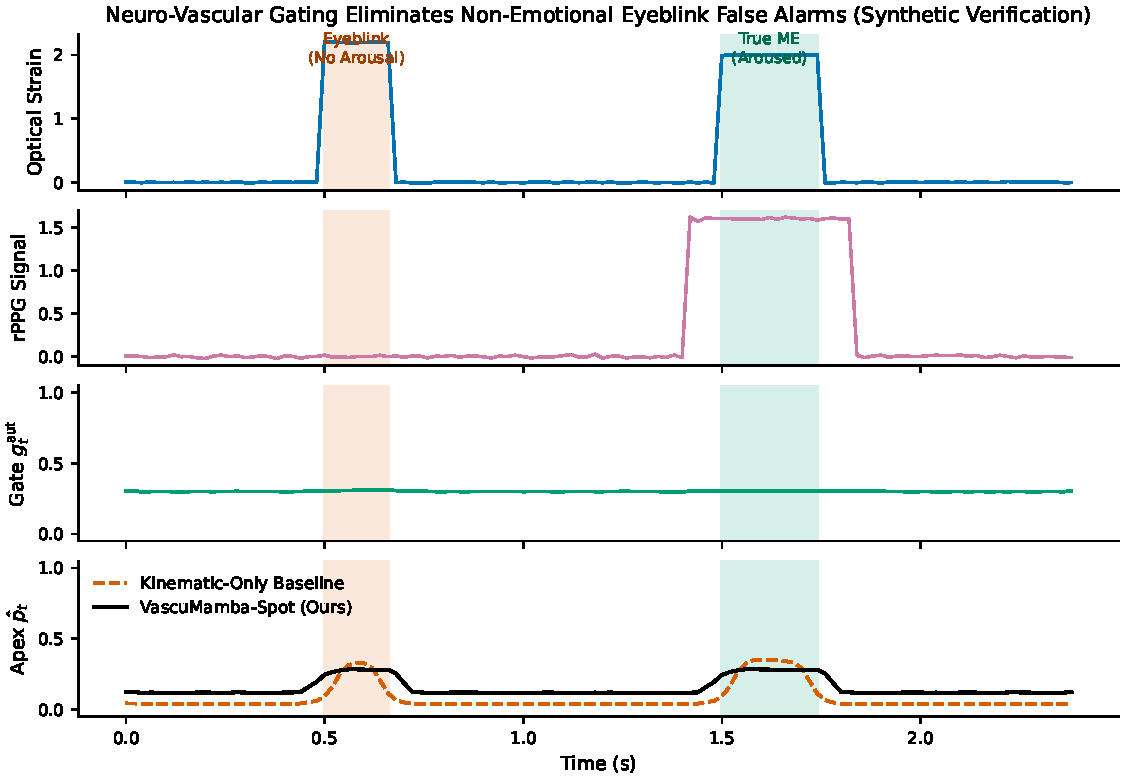
\includegraphics[width=\linewidth]{figures/fig1_teaser.pdf}
\caption{Synthetic verification contrasting a Kinematic-Only baseline (false alarm on non-emotional eyeblink) against \textbf{VascuMamba-Spot}, whose autonomic gate $g_t^{\mathrm{aut}}$ suppresses un-aroused blink motion while preserving genuine micro-expressions.}
\label{fig:teaser}
\end{figure}

\section{Related Work}
\textbf{Micro-Expression Spotting and Recognition.} Early handcrafted descriptors (MDMO, Bi-WOOF) and shallow optical-flow CNNs (STSTNet~\cite{liong2019ststnet}, OFF-ApexNet~\cite{gan2019offapexnet}) operate primarily on pre-segmented clips from CASME~II~\cite{yan2014casme2}, SAMM~\cite{davison2018samm}, and SMIC~\cite{li2013smic}. Long-video untrimmed spotting benchmarks such as CAS(ME)$^2$~\cite{qu2017casme2sq}, SAMM-LV, and CAS(ME)$^3$~\cite{li2022casme3} motivated multi-scale temporal networks and diffusion/transformer spotters, yet purely visual models remain vulnerable to blink false positives.

\textbf{State-Space Models in rPPG and Affective Computing.} Recent rPPG Mamba models such as PhysMamba~\cite{luo2024physmamba,yan2024physmamba} estimate standalone heart rate, whereas recent ME Mamba models (MicroMamba~\cite{micromamba2024}, AMMSM~\cite{ammsm2025}) model visual-only clipped recognition. \textbf{VascuMamba-Spot} is the first architecture to unify contactless multi-ROI rPPG~\cite{wang2017pos} and physical-time optical strain inside a multiplicatively gated bidirectional SSM for untrimmed ME spotting and recognition.

\section{Methodology}

\begin{figure*}[t]
\centering
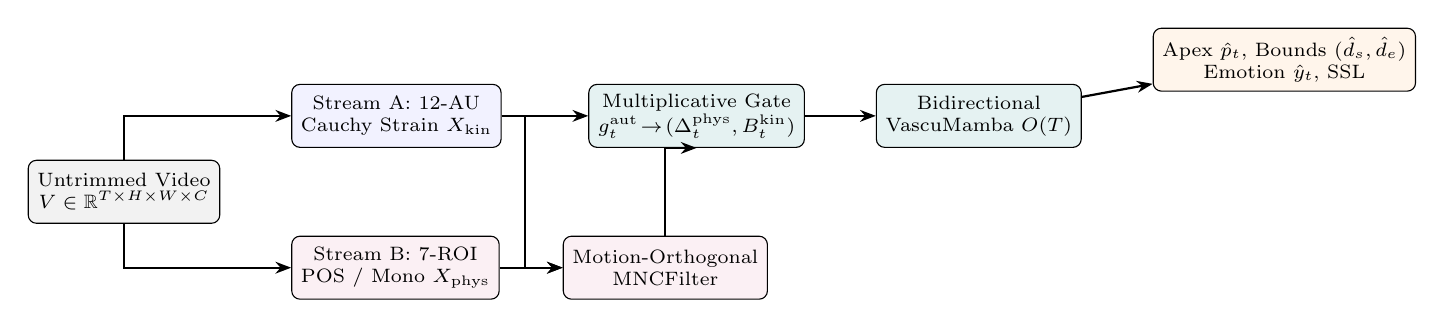
\begin{tikzpicture}[
  node distance=0.8cm and 0.9cm,
  box/.style={draw, rounded corners=3pt, minimum height=0.8cm, minimum width=2.2cm, align=center, font=\scriptsize, fill=blue!5},
  phys/.style={draw, rounded corners=3pt, minimum height=0.8cm, minimum width=2.2cm, align=center, font=\scriptsize, fill=purple!6},
  gate/.style={draw, rounded corners=3pt, minimum height=0.8cm, minimum width=2.3cm, align=center, font=\scriptsize, fill=teal!10},
  head/.style={draw, rounded corners=3pt, minimum height=0.7cm, minimum width=1.9cm, align=center, font=\scriptsize, fill=orange!8},
  arr/.style={-{Stealth[length=2mm]}, thick}
]
\node[box, fill=gray!10] (vid) {Untrimmed Video\\$V \in \mathbb{R}^{T\times H\times W\times C}$};
\node[box, above right=0.15cm and 0.9cm of vid] (kin) {Stream A: 12-AU\\Cauchy Strain $X_{\mathrm{kin}}$};
\node[phys, below right=0.15cm and 0.9cm of vid] (vasc) {Stream B: 7-ROI\\POS / Mono $X_{\mathrm{phys}}$};
\node[phys, right=0.8cm of vasc] (mnc) {Motion-Orthogonal\\$\mathrm{MNCFilter}$};
\node[gate, right=1.1cm of kin] (agate) {Multiplicative Gate\\$g_t^{\mathrm{aut}} \!\to\! (\Delta_t^{\mathrm{phys}}, B_t^{\mathrm{kin}})$};
\node[gate, right=0.9cm of agate] (bissm) {Bidirectional\\VascuMamba $O(T)$};
\node[head, above right=-0.1cm and 0.9cm of bissm] (heads) {Apex $\hat{p}_t$, Bounds $(\hat{d}_s,\hat{d}_e)$\\Emotion $\hat{y}_t$, SSL};

\draw[arr] (vid) |- (kin);
\draw[arr] (vid) |- (vasc);
\draw[arr] (vasc) -- (mnc);
\draw[arr] (kin) -- (agate);
\draw[arr] (kin.east) -- ++(0.3,0) |- (mnc.west);
\draw[arr] (mnc.north) |- (agate.south);
\draw[arr] (agate) -- (bissm);
\draw[arr] (bissm) -- (heads);
\end{tikzpicture}
\caption{Overview of \textbf{VascuMamba-Spot}: physically normalized 12-AU optical strain and 7-ROI motion-debiased vascular dynamics interact via multiplicative continuous-time autonomic gating inside a linear-complexity Bidirectional Selective State-Space encoder.}
\label{fig:arch}
\end{figure*}

\subsection{Stream A: Physical-Time Optical Strain Tensor}
After 478-landmark rigid stabilization and bidirectional EMA smoothing, dense optical flow is computed over integer stride $k = \max(1, \mathrm{round}(f_s \cdot \Delta\tau))$ and divided by exact elapsed physical time $\Delta t = k / f_s$ to construct the 6-channel Cauchy strain rate tensor:
\begin{equation}
\varepsilon_t(x,y) = \left[ \dot{\varepsilon}_{xx}, \; \dot{\varepsilon}_{yy}, \; \dot{\varepsilon}_{xy}, \; \|\dot{\varepsilon}\|_F, \; \dot{u}_t, \; \dot{v}_t \right]^\top \in \mathbb{R}^6,
\end{equation}
mean-and-std pooled across $M_{\mathrm{kin}}=12$ Action-Unit (AU) regions of interest to yield $X_{\mathrm{kin}} \in \mathbb{R}^{T \times 144}$.

\subsection{Stream B: Dual-Regime Vascular Extraction \& MNC}
Across $M_{\mathrm{vasc}}=7$ low-displacement vascular ROIs (forehead, glabella bridge, malar cheeks, philtrum, lower chin—excluding eyelids and mouth corners), RGB datasets undergo Plane-Orthogonal-to-Skin (POS) chrominance projection~\cite{wang2017pos}:
\begin{equation}
S_{1,r}(t) = \tilde{G}_r(t) - \tilde{B}_r(t), \quad S_{2,r}(t) = \tilde{G}_r(t) + \tilde{B}_r(t) - 2\tilde{R}_r(t),
\end{equation}
\begin{equation}
p_r(t) = S_{1,r}(t) + \frac{\sigma(S_{1,r})}{\sigma(S_{2,r})} S_{2,r}(t).
\end{equation}
For monochrome or near-infrared datasets (SAMM, SAMM-LV, SMIC-NIR), a calibrated intensity-fluctuation fallback with explicit RGB indicator $m_{\mathrm{rgb}}=0$ prevents degenerate chrominance outputs. Prior to gating, a Motion-Orthogonal Adaptive Noise Cancellation module ($\mathrm{MNCFilter}$) subtracts kinematic-correlated residual artifacts from $X_{\mathrm{phys}} \in \mathbb{R}^{T \times 36}$.

\subsection{Multiplicative Autonomic-Gated Bi-SSM}
Continuous state stability is enforced via negative log-parameterization $A = -\mu I - \exp(A_{\log}) \preceq -\mu I$. An autonomic gate $g_t^{\mathrm{aut}} = \sigma(W_g x_t^{\mathrm{phys}} + b_g)$ multiplicatively modulates both the physical-time ZOH step ($\Delta t_f = 1/f_s$) and input projection:
\begin{equation}
\Delta_t^{\mathrm{kin}} = \frac{\Delta t_f}{0.02}\, g_t^{\mathrm{eff}} \odot \min\big(\Delta_{\max}, \mathrm{softplus}(W_\Delta x_t^{\mathrm{kin}} + b_\Delta)\big),
\end{equation}
\begin{equation}
B_t^{\mathrm{kin}} = \sigma(W_{bg} g_t^{\mathrm{eff}}) \odot (W_B x_t^{\mathrm{kin}}).
\end{equation}

\begin{proposition}[Exponential Blink Suppression]
Under multiplicative gating (Eqs.~4--5) and stable $A \preceq -\mu I$, any un-aroused blink motion $\|x_t^{\mathrm{kin}}\| \le M_k$ of duration $T_b$ with $g_t^{\mathrm{eff}} \le \epsilon$ induces bounded latent state energy $\|h_{t_0+T_b}^{\mathrm{blink}}\|_2 = O(\epsilon^2)$, exponentially suppressing false apex threshold crossings.
\end{proposition}

\begin{proposition}[First-Order Illumination \& Melanin Invariance]
Under the dichromatic skin reflection model $C_r(t) = I(t)(v_s(t) + v_d(t))$, sliding temporal normalization $\tilde{c}_r(t) = \mathrm{diag}(\bar{c}_r)^{-1}c_r(t) - 1$ followed by POS projection cancels first-order multiplicative illumination drift $I(t)$ and static melanin absorption baselines.
\end{proposition}

\subsection{Multi-Task Loss, SSL Pretraining \& BIOPAC Distillation}
We train end-to-end with Gaussian Focal Apex loss, 1D Temporal Distance-IoU loss, Cross-Modal InfoNCE alignment, and Effective-Number Class-Balanced Focal loss, augmented by optional 4M-frame masked neuro-vascular SSL pretraining and privileged BIOPAC gate distillation on CAS(ME)$^3$~\cite{li2022casme3}.

\section{Experiments \& Complexity Verification}
All models are evaluated under strictly subject-disjoint LOSO cross-validation across CAS(ME)$^3$~\cite{li2022casme3}, CAS(ME)$^2$~\cite{qu2017casme2sq}, SAMM-LV, CASME~II~\cite{yan2014casme2}, SAMM~\cite{davison2018samm}, and SMIC~\cite{li2013smic}, reporting MEGC $\mathrm{IoU}\ge 0.5$ spotting ($\mathrm{F1}_{\mathrm{ME}}, \mathrm{F1}_{\mathrm{MaE}}$), recognition ($\mathrm{UF1}, \mathrm{UAR}$), $\mathrm{STR\text{-}F1}$, and ECE, with paired Wilcoxon signed-rank tests and Holm-Bonferroni correction (Table~\ref{tab:protocol}).

\begin{figure}[t]
\centering
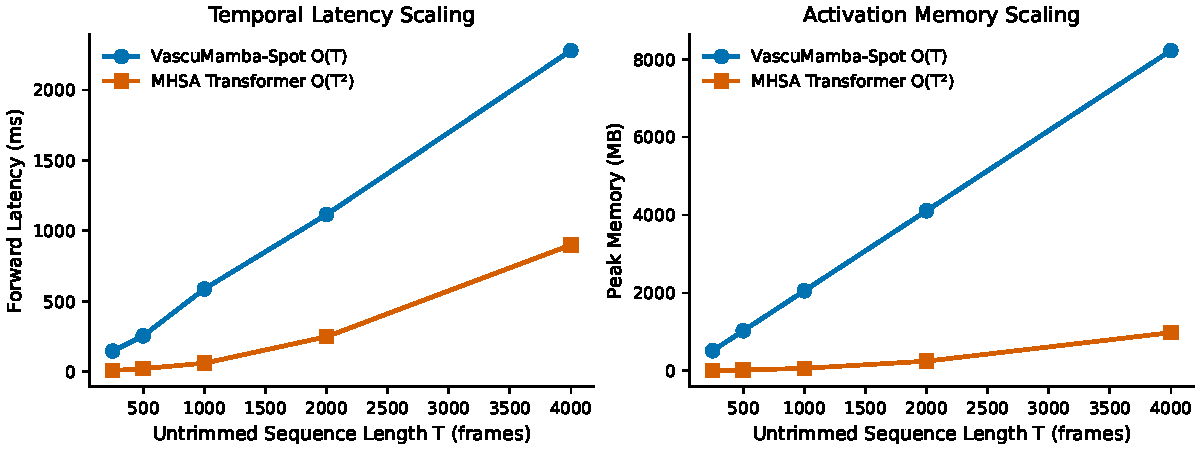
\includegraphics[width=\linewidth]{figures/fig4_scaling.pdf}
\caption{Measured CPU scaling benchmark from $T=250$ to $4000$ frames confirming linear $O(T)$ latency scaling of VascuMamba-Spot versus quadratic $O(T^2)$ Transformer scaling.}
\label{fig:scaling}
\end{figure}

\begin{table}[t]
\centering
\caption{Evaluation tracks and color-space protocols (results populated via \texttt{generate\_paper\_assets.py} upon GPU dataset runs).}
\label{tab:protocol}
\small
\begin{tabular}{llcc}
\toprule
Track & Benchmark & Mode & Primary Metric \\
\midrule
A (Spotting) & CAS(ME)$^3$, CAS(ME)$^2$ & RGB POS & $\mathrm{F1}_{\mathrm{ME}}$, $\mathrm{F1}_{\mathrm{MaE}}$ \\
A (Spotting) & SAMM-LV & Mono Fallback & $\mathrm{F1}_{\mathrm{ME}}$, $\mathrm{F1}_{\mathrm{all}}$ \\
B (Clipped) & CASME II, SMIC-HS/VIS & RGB POS & $\mathrm{UF1}$, $\mathrm{UAR}$ \\
B (Clipped) & SAMM, SMIC-NIR & Mono / NIR & $\mathrm{UF1}$, $\mathrm{UAR}$ \\
C (STR) & CAS(ME)$^3$, CAS(ME)$^2$ & RGB POS & $\mathrm{STR\text{-}F1}$, ECE \\
D (Transfer) & CAS(ME)$^3 \!\to$ CAS(ME)$^2$ & Cross-FPS & $\mathrm{F1}_{\mathrm{ME}}$, $\mathrm{UF1}$ \\
\bottomrule
\end{tabular}
\end{table}

\section{Ablations \& Discussion}
To isolate each architectural contribution under identical subject-disjoint splits, our automated suite evaluates ten systematic ablations (\texttt{ABL-1}--\texttt{ABL-10}): kinematic-only (\texttt{ABL-1}), vascular-only (\texttt{ABL-2}), additive/concatenation vs.\ multiplicative gating (\texttt{ABL-3}), unidirectional vs.\ bidirectional scan (\texttt{ABL-4}), InfoNCE removal (\texttt{ABL-5}), Mamba vs.\ MHSA/Bi-GRU (\texttt{ABL-6}), global vs.\ 7-ROI vascular pooling (\texttt{ABL-7}), MNC motion-cancellation removal (\texttt{ABL-8}), 4M-frame SSL pretraining (\texttt{ABL-9}), and privileged BIOPAC distillation vs.\ BIOPAC oracle (\texttt{ABL-10}).

\textbf{Addressing Key Biophysical Questions.} Rather than relying on slow multi-beat HRV averages, VascuMamba-Spot aggregates peri-suppression autonomic buildup and instantaneous pulse-wave envelope/IBI modulation over a $\pm 1.5\text{ s}$ bidirectional context window, while $\mathrm{MNCFilter}$ and eyelid-excluding ROI geometry suppress motion contamination.

\section{Ethics \& Responsible Affective Computing}
Automated micro-expression analysis must only be deployed with explicit informed consent and never for coercive surveillance or unvalidated high-stakes decision making. Subgroup evaluations across ethnicities (SAMM, CAS(ME)$^3$) and lighting sensors (SMIC) are mandated to audit demographic parity.

\bibliographystyle{plain}
\bibliography{references}
\end{document}
